\documentclass[10pt,a4paper]{article}
\usepackage[utf8]{inputenc}
\usepackage[english]{babel}
%\usepackage{minted}
\usepackage{listings}
\usepackage{xcolor}
\usepackage{graphicx}

%For syntax highlighting
\definecolor{codegreen}{rgb}{0,0.6,0}
\definecolor{codegray}{rgb}{0.5,0.5,0.5}
\definecolor{codepurple}{rgb}{0.58,0,0.82}
\definecolor{backcolour}{rgb}{1,1,1}

%%Sets different parameters
\lstdefinestyle{mystyle}{
	backgroundcolor=\color{backcolour},   
    commentstyle=\color{codegreen},
    keywordstyle=\color{magenta},
    numberstyle=\tiny\color{codegray},
    stringstyle=\color{codepurple},
    basicstyle=\ttfamily\footnotesize,
    breakatwhitespace=false,         
    breaklines=true,                 
    captionpos=b,                    
    keepspaces=true,                 
    numbers=left,                    
    numbersep=5pt,                  
    showspaces=false,                
    showstringspaces=false,
    showtabs=false,                  
    tabsize=4
}
\lstset{style=mystyle}

\title{\bf Display System date and time}
\author{\vspace{-10ex}}
\date{\vspace{-10ex}}
\begin{document}
\maketitle

\begin{minipage}{0.45\textwidth}
        \begin{tabular}{l l}
            \textbf{Expt No:}&11\\
            \textbf{Date :}&16/10/2020
        \end{tabular}
\end{minipage}%
\begin{minipage}{0.45\textwidth}
        \begin{tabular}{l l}
             \textbf{Name:}& Shivanirudh S G  \\
             \textbf{Reg No:} & 185001146 
        \end{tabular}
\end{minipage}
\vspace{1cm}
\hrule

\begin{flushleft}
\subsection*{\textbf{Aim:}} 
To display system date and time in 8086.

\vspace{1cm}
\hrule
\subsection*{\textbf{\underline{System date}}}

\subsubsection*{\textbf{Algorithm:}}
\begin{itemize}
    \item Move the data segment to the AX register and then move it to the DS register.
    \item Move value 2AH to AH register.
    \item Move offset of day into SI register, and move value of DL register into SI.
    \item Move offset of month into SI register, and move value of DH register into SI.
    \item Move offset of year into SI register, and move value of CX register into SI.
\end{itemize}

\newpage
\subsubsection*{\textbf{Program:}}

\begin{table}[htb]
\centering
\resizebox{\columnwidth}{!}{
\begin{tabular}{|l|l|} 
\hline
\textbf{Program}                                                 & \textbf{Comments}                             \\ 
\hline
\hline
assume cs:code, ds:data                                          & Declare code and data segments                \\
\hline
data segment                                                     & Start of data segment                         \\
\hline
day db 01 dup(?)                                                 & Define byte day for day of month              \\
\hline  
month db 01 dup(?)                                               & Define byte month for month                   \\
\hline
year db 02 dup(?)                                                & Define word year for year                     \\
\hline
data ends                                                        & End of data segment                           \\
\hline
code segment                                                     & Start of code segment                         \\
\hline
start:~mov ax, data                                              & Move data to AX register                      \\
\hline
mov ds, ax                                                       & Move contents of AX register to DS register   \\
\hline
mov ah, 2ah                                                      & Move value 2AH into AH register               \\
\hline
int 21h                                                          & Request interrupt 21H to capture system date  \\
\hline
mov si, offset day                                               & Move offset of day into SI register           \\
\hline
mov [si], dl                                                     & Move value in DL to address at [SI]           \\
\hline
mov si, offset month                                             & Move offset of month into SI register         \\
\hline
mov [si], dh                                                     & Move value in DH to address at [SI]           \\
\hline
mov si, offset year                                              & Move offset of year into SI register          \\
\hline
mov [si], cx                                                     & Move value in CX to address at [SI]           \\
\hline
mov ah, 4ch                                                      & To request interrupt                          \\
\hline
int 21h                                                          & Request interrupt routine                     \\ 
\hline
code ends                                                        & End of code segment                           \\
\hline
end start                                                        &                                               \\
\hline
\end{tabular}
}
\end{table}

\newpage
\subsection*{\textbf{Unassembled code:}}
\begin{figure}[h]
    \centering
    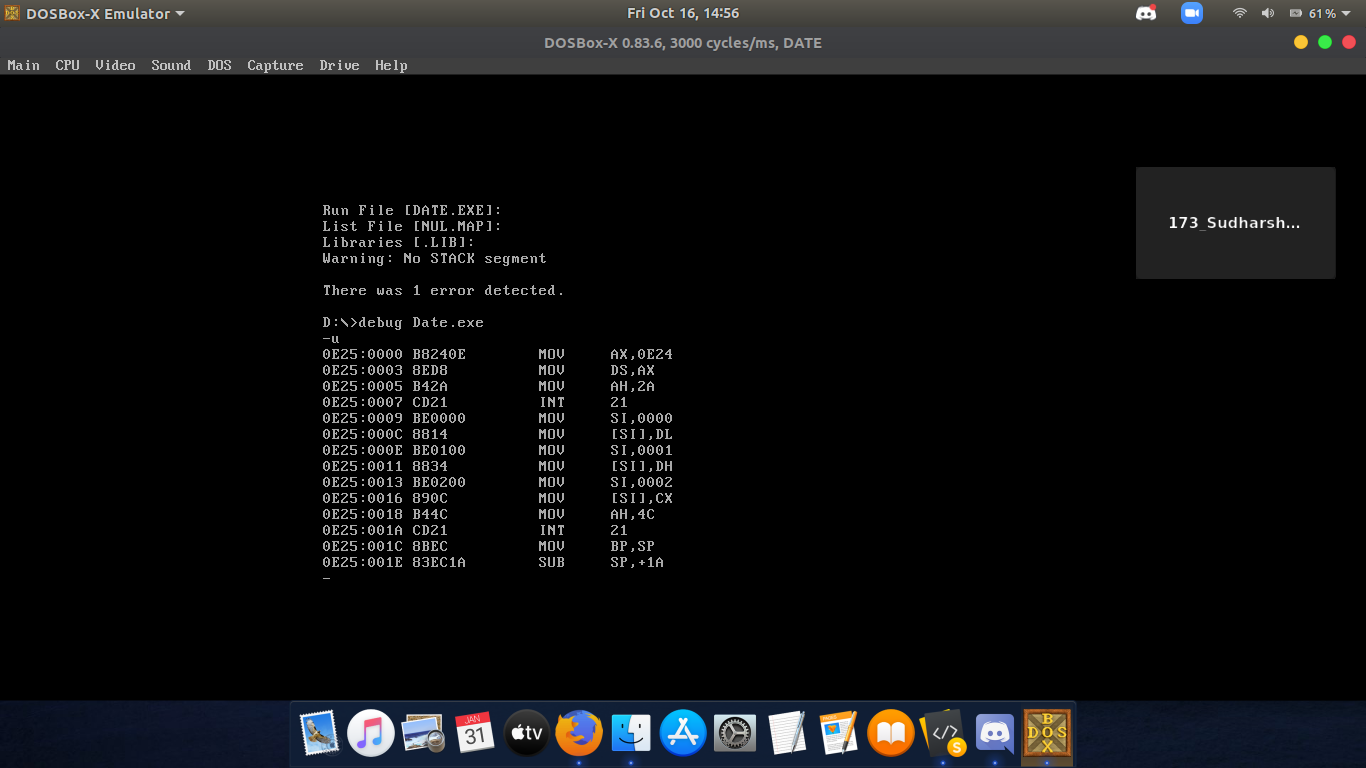
\includegraphics[trim = 100mm 60mm 200mm 110mm, clip, width = \textwidth]{Pics/DateUS.png}
\end{figure}
\subsubsection*{\textbf{Input and Output:}}
\begin{figure}[h]
    \centering
    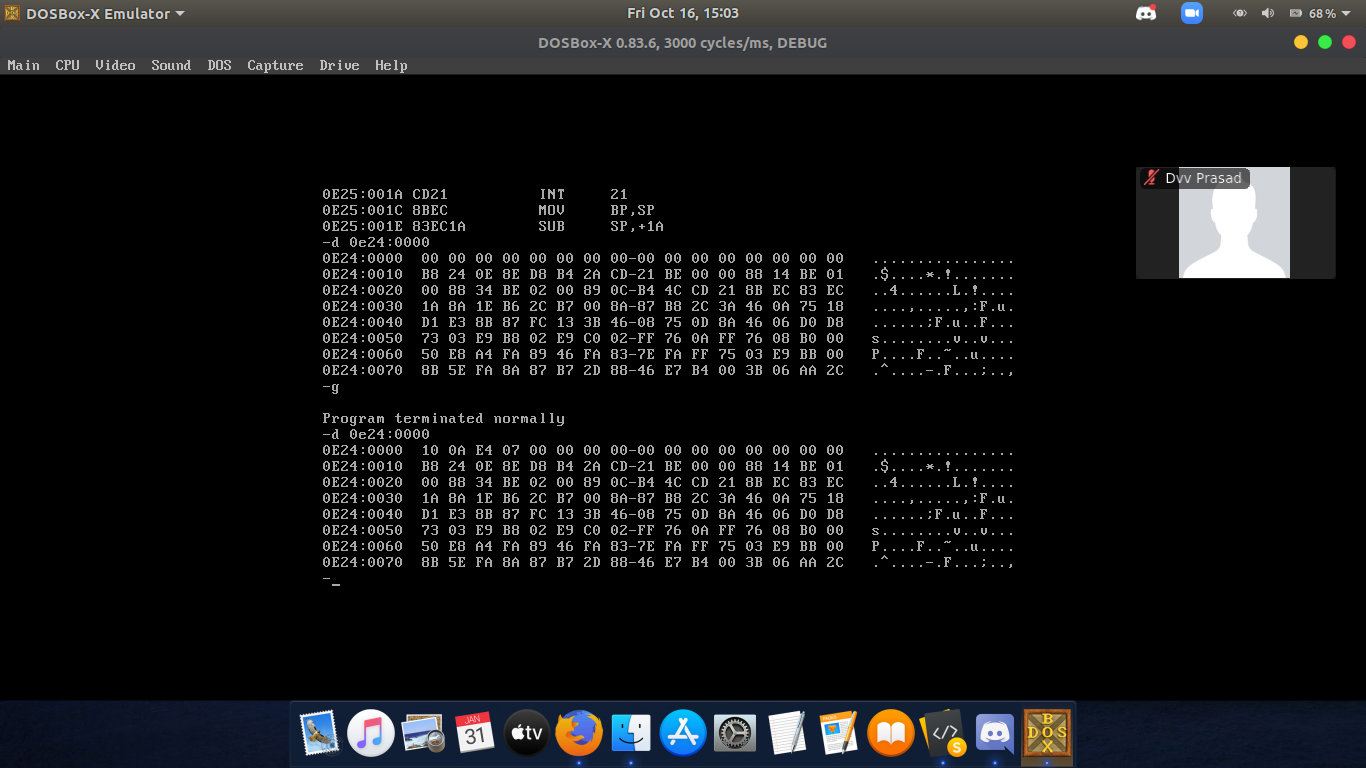
\includegraphics[trim = 100mm 60mm 100mm 150mm, clip, width = \textwidth]{Pics/DateIO.png}
    \caption{\textbf{Output:} 16 10 2020 \textbf{in hex:} 10 0A 07E4}
\end{figure}
%-------------------------------------------------------------------------------------------------------------------------------------------
\hrule
\newpage
\subsection*{\textbf{\underline{System time}}}

\subsubsection*{\textbf{Algorithm:}}
\begin{itemize}
    \item Move the data segment to the AX register and then move it to the DS register.
    \item Move value 2CH to AH register.
    \item Move offset of hour into SI register, and move value of CH register into SI.
    \item Move offset of min into SI register, and move value of CL register into SI.
    \item Move offset of sec into SI register, and move value of DH register into SI.
\end{itemize}

\newpage
\subsubsection*{\textbf{Program:}}

\begin{table}[htb]
\centering
\resizebox{\columnwidth}{!}{
\begin{tabular}{|l|l|} 
\hline
\textbf{Program}                                                 & \textbf{Comments}                             \\ 
\hline
\hline
assume cs:code, ds:data                                          & Declare code and data segments                \\
\hline
data segment                                                     & Start of data segment                         \\
\hline
hour db 01 dup(?)                                                & Define byte hour for hour of day              \\
\hline  
min db 01 dup(?)                                                 & Define byte min for minutes                   \\
\hline
sec db 01 dup(?)                                                 & Define word sec for seconds                   \\
\hline
data ends                                                        & End of data segment                           \\
\hline
code segment                                                     & Start of code segment                         \\
\hline
start:~mov ax, data                                              & Move data to AX register                      \\
\hline
mov ds, ax                                                       & Move contents of AX register to DS register   \\
\hline
mov ah, 2ch                                                      & Move value 2CH into AH register               \\
\hline
int 21h                                                          & Request interrupt 21H to capture system date  \\
\hline
mov si, offset hour                                              & Move offset of hour into SI register          \\
\hline
mov [si], ch                                                     & Move value in CH to address at [SI]           \\
\hline
mov si, offset min                                               & Move offset of min into SI register           \\
\hline
mov [si], cl                                                     & Move value in CL to address at [SI]           \\
\hline
mov si, offset sec                                               & Move offset of sec into SI register           \\
\hline
mov [si], dh                                                     & Move value in DH to address at [SI]           \\
\hline
mov ah, 4ch                                                      & To request interrupt                          \\
\hline
int 21h                                                          & Request interrupt routine                     \\ 
\hline
code ends                                                        & End of code segment                           \\
\hline
end start                                                        &                                               \\
\hline
\end{tabular}
}
\end{table}

\newpage
\subsection*{\textbf{Unassembled code:}}
\begin{figure}[h]
    \centering
    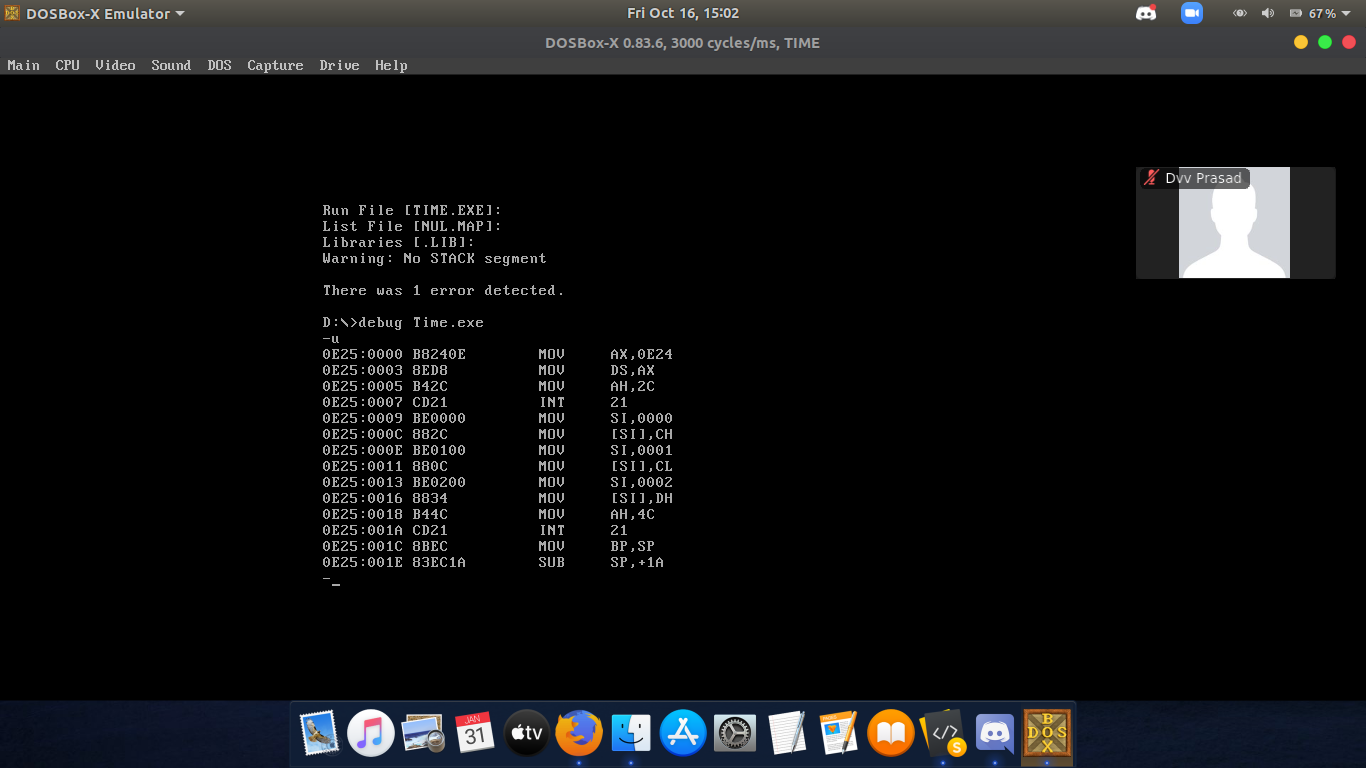
\includegraphics[trim = 100mm 60mm 200mm 110mm, clip, width = \textwidth]{Pics/TimeUS.png}
\end{figure}
\subsubsection*{\textbf{Input and Output:}}
\begin{figure}[h]
    \centering
    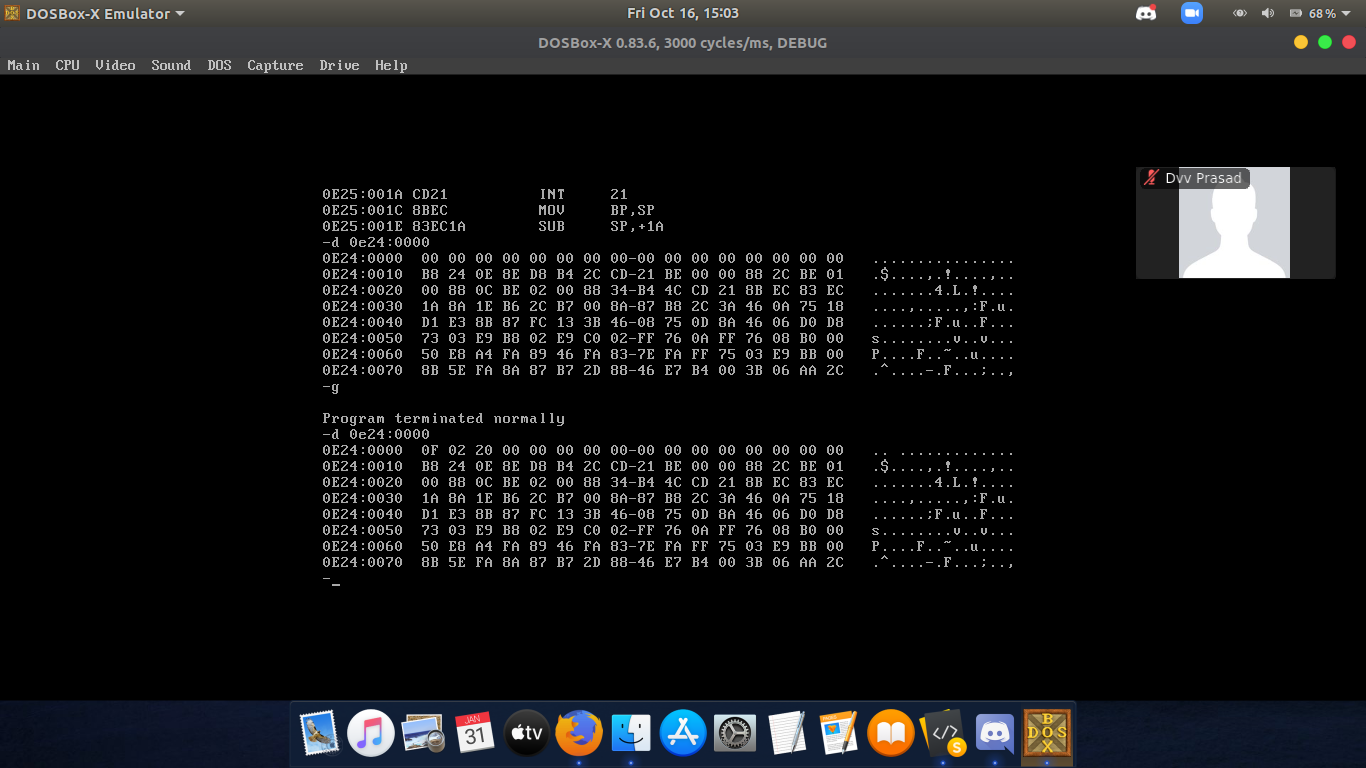
\includegraphics[trim = 100mm 60mm 100mm 150mm, clip, width = \textwidth]{Pics/TimeIO.png}
    \caption{\textbf{Output:} 15 02 32 \textbf{in hex:} 0F 02 20}
\end{figure}
\hrule
\subsection*{\textbf{Result:}}
The 8086 programs were written to display system date and time, and the results observed.
\end{flushleft}
\end{document}